\section{Auswertung}
\ref{sec:aus}

\subsection{Dampfdruckkurve Tiefdruck}
Zunächst wird die Dampfdruckkurve für Drücke im Bereich von 30 $\si{\milli\bar}$ bis circa 1000 $\si{\milli\bar}$ untersucht. Das Vorgehen wird in \autoref{} beschrieben.
Die aufgenommenen Messwerte sind in der \autoref{tab:1} aufgelistet.

\begin{table}
    \centering
    \caption{Messwerte vom Druck $p$, sowie der Wassertemperatur $T_W$ und der Lufttemperatur $T_L$ }
    \label{tab:1}
    \begin{tabular} {S[table-format=2.0] S[table-format=3.1] S[table-format=3.0]}
        \toprule
        {$p \mathbin{/} \si{\milli\bar}$}&{$T_W \mathbin{/} \si{\celsius}$} & {$T_L \mathbin{/} \si{\celsius}$} \\
    \midrule
    74  & 30   &   25   \\
    86  & 35   &   36   \\
    96  & 40   &   38   \\
    110 & 45   &   40   \\
    127 & 50   &   49   \\
    160 & 55   &   54   \\
    200 & 60   &   59.5 \\
    247 & 65   &   64   \\
    307 & 70   &   70   \\
    372 & 75   &   71   \\
    460 & 80   &   82   \\
    550 & 85   &   99   \\
    648 & 90   &   106.5\\
    \bottomrule
\end{tabular}
\end{table}

\noindent
Die gemessenen Werte werden in ein Diagramm (\ref{fig:1}) eingetragen und mithilfe einer Augleichsgeraden der Form
\begin{equation}
    y = m*x + n 
\end{equation}

\noindent
gefittet, wobei sich mit der \autoref{} %Logerithmus
für $m=-\frac{L}{R}$ und für $y=\frac{p}{p_0}$ ergibt. 

\begin{figure}
    \centering
    \caption{Messdaten und Fit für die Temperatur gegen den Druck}
    \label{fig:hochdruck}
    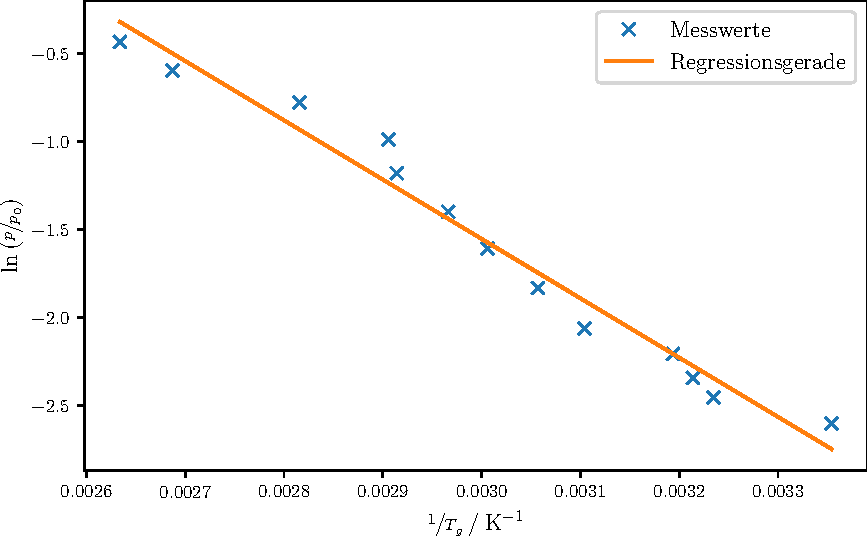
\includegraphics{Daten/tiefdruck.pdf}
\end{figure}

\noindent
Mithilfe der Ausgleichsgerade ergibt sich für 
\begin{align*}
    m &= \SI{-3369.90(17463)}{\kelvin}\\
    b &= \SI{0.65(53)} \, .
\end{align*}

\noindent 
Daraus lässt sich die Verdampfungswärme $L$ mithilfe der Gaskonstante $R = \SI{8,314462618}{\joule\per\mole\per\kelvin}$\cite{gasconstant} errechnen zu 
\begin{equation*}
    L = \SI{2.80(15)e04}{\joule\per\mole} \, .
\end{equation*}

